\documentclass[12pt]{article}

% Packages for math and TikZ
\usepackage{amsmath, amssymb}
\usepackage{tikz}
\usetikzlibrary{arrows, positioning, calc}

% For better spacing and professional layout
\usepackage[margin=1in]{geometry}
\usepackage{hyperref}
\usepackage{lipsum} % For dummy text if needed

\begin{document}

\section*{The Exact Mathematical Definition of a Function}

A \textbf{function} $f$ from a set $A$ to a set $B$, written as
\[
f: A \to B,
\]
is defined as a relation that assigns to each element $a \in A$ \emph{exactly one} element $b \in B$. More formally, $f$ is a subset of the Cartesian product $A \times B$ with the property that for every $a \in A$, there exists a unique $b \in B$ such that 
\[
(a,b) \in f.
\]
This uniqueness is essential: it means that an element in the domain cannot be assigned more than one output in the codomain.

\subsection*{Motivation from Finite and Infinite Perspectives}

\textbf{1. Finite Table Representation:}

When the domain $A$ is finite, a function can be completely described by a table that lists each input and its corresponding output. For example, consider the function 
\[
f: \{1,2,3\} \to \{a,b,c\}
\]
given by:
\[
\begin{array}{c|c}
a \in A & f(a) \in B \\
\hline
1 & a \\
2 & b \\
3 & c \\
\end{array}
\]
The following TikZ diagram illustrates this mapping:

\begin{center}
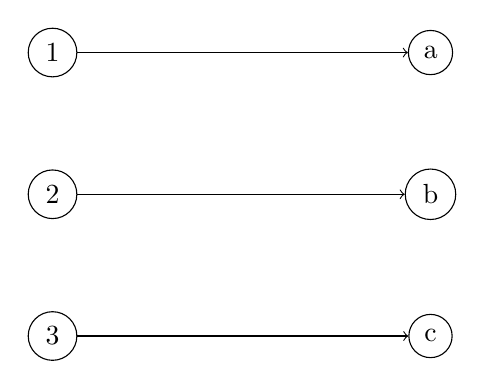
\begin{tikzpicture}[node distance=1.8cm, auto]
% Domain nodes
\node (A1) [draw, circle] {1};
\node (A2) [draw, circle, below of=A1] {2};
\node (A3) [draw, circle, below of=A2] {3};

% Codomain nodes
\node (B1) [draw, circle, right of=A1, xshift=3cm] {a};
\node (B2) [draw, circle, right of=A2, xshift=3cm] {b};
\node (B3) [draw, circle, right of=A3, xshift=3cm] {c};

% Arrows showing the mapping
\draw[->] (A1) -- (B1);
\draw[->] (A2) -- (B2);
\draw[->] (A3) -- (B3);
\end{tikzpicture}
\end{center}

This table and diagram clearly show that each input from the set $\{1,2,3\}$ is paired with a unique output.

\vspace{0.5cm}
\textbf{2. Infinite Function Expression:}

When the domain $A$ is infinite, such as $A = \mathbb{R}$, it is impractical to list all the pairs. Instead, a function is described by a rule or formula. For example, consider the function 
\[
f: \mathbb{R} \to \mathbb{R}, \quad f(x) = x^2.
\]
This single formula compactly describes an infinite number of input-output pairs. The following TikZ diagram gives a conceptual visualization of this idea:

\begin{center}
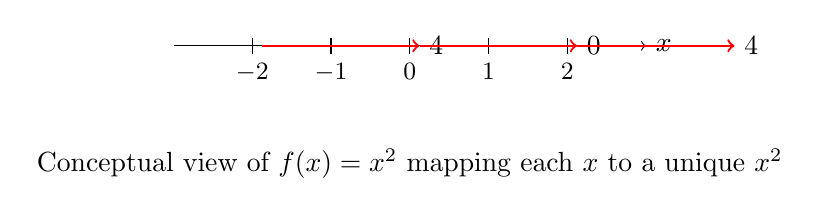
\begin{tikzpicture}[node distance=1.5cm, auto]
% Domain number line
\draw[->] (-3,0) -- (3,0) node[right] {$x$};
\foreach \x in {-2,-1,0,1,2} {
\draw (\x,0.1) -- (\x,-0.1) node[below] {\small $\x$};
}

% A few sample points and arrows for the mapping
\node (P1) at (-2,0) {};
\node (Q1) [right=2cm of P1] {$4$};

\node (P2) at (0,0) {};
\node (Q2) [right=2cm of P2] {$0$};

\node (P3) at (2,0) {};
\node (Q3) [right=2cm of P3] {$4$};

\draw[->, red, thick] (P1) -- (Q1);
\draw[->, red, thick] (P2) -- (Q2);
\draw[->, red, thick] (P3) -- (Q3);

% Label for function
\node at (0,-1.5) {Conceptual view of $f(x)=x^2$ mapping each $x$ to a unique $x^2$};
\end{tikzpicture}
\end{center}

\vspace{0.5cm}
\textbf{Why the Definition Must be This Way:}

\begin{itemize}
\item \emph{Uniqueness:} The requirement that each $a \in A$ is assigned exactly one $b \in B$ ensures that the function behaves predictably—knowing the input fully determines the output.
\item \emph{Consistency Across Finite and Infinite Cases:} Whether a function is given by a finite table or by an infinite rule, the concept remains the same: a well-defined assignment of outputs to inputs.
\item \emph{Foundational Role:} This strict definition underpins much of mathematics. It ensures that functions can be composed, inverted (when appropriate), and analyzed in a rigorous manner.
\end{itemize}

\bigskip
\textbf{Conclusion:}  
The exact definition of a function—requiring that every input is paired with a unique output—is motivated by the need for consistency, predictability, and clarity. Finite tables and infinite formulas are simply two perspectives on the same fundamental concept.

\end{document}
